% How to use writeLaTeX: 
%
% You edit the source code here on the left, and the preview on the
% right shows you the result within a few seconds.
%
% Bookmark this page and share the URL with your co-authors. They can
% edit at the same time!
%
% You can upload figures, bibliographies, custom classes and
% styles using the files menu.
%
%%%%%%%%%%%%%%%%%%%%%%%%%%%%%%%%%%%%%%%%%%%%%%%%%%%%%%%%%%%%%%%%%%%%%%

\documentclass[12pt,english,brazil]{article}
\usepackage{sbc-template}
\usepackage{adjustbox}
\usepackage{graphicx,url}
\usepackage{graphics}
\usepackage{color}
\usepackage{colortbl}
\usepackage[utf8]{inputenc}  
% Coloquei esse pacote para tamanho pequeno de fonte
\usepackage{scalefnt}
\usepackage{multirow}
\usepackage{subfigure}
\usepackage{multicol}
\usepackage{babel}
\babeltags{br = brazil, en = english}
\usepackage[T1]{fontenc}
\usepackage{xspace}
\usepackage{url}
\usepackage{enumerate}

\usepackage{xargs}
\usepackage[colorinlistoftodos,prependcaption,textsize=tiny]{todonotes}
\newcommandx{\ups}[2][1=]{\todo[linecolor=red,backgroundcolor=red!25,bordercolor=red,#1]{\tiny Gerson: #2}\xspace}
\newcommandx{\aham}[2][1=]{\todo[linecolor=yellow,backgroundcolor=yellow!25,bordercolor=yellow,#1]{\tiny Gui: #2}\xspace}
     
\sloppy

\title{Estudo de viabilidade do uso de Raspberry como servidor R-Shiny}

\author{Guilherme de Souza\inst{1}}


\address{Programa de Pós-Graduação em Computação \\Universidade Federal de Pelotas (UFPel)\\
  Caixa Postal 354 -- 96010.610 -- Pelotas -- RS -- Brazil
\nextinstitute
  Instituto de Matemática e Estatística (IME) -- Universidade de São Paulo (USP)\\
  Rua do Matão, 1010 -- São Paulo -- SP -- Brazil
  \email{\{gdsdsilva,gerson.cavalheiro\}@inf.ufpel.edu.br, gold@ime.usp.br}
}

\begin{document} 

\maketitle
    
\en
\begin{abstract}
The use of servers is widespread in practically all computing areas. Notwithstanding this, the concern with the search for solutions aimed at reducing energy use is also a reality. In this article, we present the use of a Small Business Computer (SLC), the Raspberry-Pi, as a low-cost alternative to provide application server services developed using the R language together with R-Shiny. To do so, a Raspberry Pi device was configured and compared to its performance, with an X64 architecture server. Scenarios and performance testing tools were applied and, through these, it was possible to evaluate and verify that the small board supports serving a low number of users without the use of any tuning technique, thus confirming the veracity of the initially proposed premise .

\end{abstract}

\br
\begin{resumo} (rascunho por Giovani)
O uso de servidores esta difundido em praticamente todas as áreas computacionais. Não obstante a isso, a preocupação com a busca de soluções atentas à redução do uso de energia, também é uma realidade.  Apresentamos neste artigo o uso de um Small Business Computer (SLC), o Raspberry Pi, como uma alternativa de baixo custo para prover serviços de servidor de aplicação desenvolvida utilizando a linguagem R juntamente com R-Shiny. Para tal, um dispositivo Raspberry Pi foi configurado e confrontado quanto a sua performance, com um servidor de arquitetura X64. Cenários e ferramentas de testes de desempenho foram aplicados e, por meio destes, pôde-se avaliar e constatar que a \emph{small board} suporta atender um baixo número de usuários sem a utilização de quaisquer técnica de \emph{tuning}, assim, confirmando a veracidade da premissa inicialmente proposta.


\end{resumo}



\section{Introdução}

A decisão por realizar, ou não, um investimento financeiro passa, muitas vezes, pela análise de uma grande
massa de dados. Os setores agrícolas e de obras civis possuem situações onde esta análise tem relevada importância, considerando aspectos hidrológicos. No contexto da agricultura, a decisão
por uma cultura, pelo agricultor, ou pela taxa de juros a ser aplicada, por uma entidade voltada ao
financiamento rural, depende da análise, entre outros, dos regimes hídricos do local onde a plantação ou
a aplicação dos recursos será realizada. Dependente também da análise dos regimes hídricos dependem
decisões sobre implantação de infraestruturas civis, como pontes, barragens para reservatórios aquíferos
ou geração de energia e mesmo para dimensionamento de telhados de imóveis. A pura visualização de
grande massas dados, por si, é complexa. Torna-se ainda mais complexa quando a visualização depende
do tratamento dos dados segundo modelos que regem a análise do problema a ser considerado.

Para atender a necessidade de análise da grande massa de dados associadas aos aspectos hídricos, foi desenvolvida a aplicação WebSYHDA \cite{syhda}. O WebSYHDA é uma ferramenta, disponibilizada na Web, para aplicação de modelos hídricos e apresentação de gráficos com o resultado destes. A
ferramenta oferece um conjunto de recursos que permite a aplicação de diferentes modelos hídricos sobre
séries temporais registrando dados como móveis de rios, vazão e índices de precipitação. O WebSYHDA
foi desenvolvido em R, com apoio do pacote de visualização Shiny. Implantado em um servidor R, essa
ferramenta foi projetada para atender diferentes usuários simultaneamente.

Enquanto um serviço R, o suporte de operação do WebSYHDA é realizado de forma convencional pelo servidor Shinyapps.io\footnote{Shinyapps.io: \url{https://www.shinyapps.io/}} . Nessa etapa do trabalho busca-se avaliar as necessidades de
estrutura física para suportar esse serviço. O presente artigo avalia a escalabilidade em termos de número
de usuários WebSyhda ativos simultaneamente em dois modelos de arquitetura: um servidor convencional
e um dispositivo de borda (\emph{small board}). No contexto do trabalho realizado, as métricas de desempenho, que são valores brutos que provem a base para alguma forma de pesquisa ou estudo e podem ser compostos por valores de diversas categorias e formato, tem a finalidade de quantificar objetivamente as funções de coletas de dados de avaliação e desempenho.
O caso de estudo encaminhado considera o serviço WebSYHDA, desenvolvido com a finalidade de processamento complexo de séries hidrológicas. São consideradas duas plataformas de suporte: um servidor com arquitetura convencional e um dispositivo de baixa capacidade (\emph{small board}). 
%O objetivo deste estudo é identificar componentes do software, atualmente construído de forma monolítica, na forma de microserviços.

O presente artigo está organizado da seguinte forma: na Seção~\ref{sec:TrabalhosRelacionados} serão apresentados trabalhos relacionados, na Seção~\ref{sec:websyhda} é apresentada a aplicação utilizada como \emph{benchmark}. A Seção~\ref{sec:metodologia} são apresentadas as ferramentas utilizadas para realização dos experimentos. Na Seção~\ref{sec:Resultados}, são descritos os resultados obtidos considerando os cenários representativos. As considerações finais e trabalhos futuros se encontram na Seção~\ref{sec:conlusao}.

\section{Trabalhos Relacionados} \label{sec:TrabalhosRelacionados}

O estudo da escalabilidade de servidores no atendimento aos usuários é constante na literatura \cite{generic1}, \cite{generic5}, \cite{generic3}, \cite{generic4}. Nos últimos anos, esse estudo passou a incluir a análise das questões
energéticas \cite{generic6}, \cite{generic7}, \cite{generic8}. Neste contexto, o uso de dispositivos de borda, os chamados \emph{small
boards}, em substituição a servidores convencionais tem se apresentado como alternativa. No estudo de caso documento neste artigo, é considerada uma aplicação desenvolvida sob um servidor R.

Inicialmente, com um propósito similar ao WebSYHDA, no que tange ao uso de R e a estrutura Shiny, cita-se o  trabalho de \cite{CIPR} que utiliza os referidos recursos para criar uma aplicação web denominada \emph{Cluster Identity PRedictor}\footnote{Cluster Identity PRedictor: \url{https://github.com/atakanekiz/CIPR-Package}} (CIPR), que fornece uma interface gráfica de usuário para pontuar perfis de expressão gênica de \emph{clusters} de células.
Em outro contexto, a finalidade de criar um servidor de arquivos utilizando um Raspberry Pi, para guardar os dados e poder compartilhar na rede, fora objeto de estudo de Bruschi (2016). Este concluiu que o dispositivo pode ser utilizado com o propósito em questão, com economia de custos sem, contudo, deixar de ser viável para esta aplicação, observando-se apenas algumas variações de desempenho dependendo do tipo de armazenamento.

A Raspberry Pi também foi utilizado, conforme Azevedo (2019), para propor a viabilidade de sua utilização em hospedar um honeypot, mostrando que sua efetividade irá depender da eficiência do software utilizado e também do tamanho e complexidade da rede em que ficará esse dispositivo, para dar efetividade ao objetivo proposto. Também dentro desse contexto de propor funcionalidades "servers" ao Raspberry Pi, Rafael et al (2013), outrora já mostrara que o uso de um computador de baixo custo - o Raspberry-Pi, pode ser usado de forma segura como um servidor web,  propiciando economia de energia.

[Oliveira and Ataides 2017] propôs avaliar a substituição do hardware convencional por um hardware de baixo consumo que respeite o Service-Level-Agreement (SLA) e reduza o consumo de energia dos data centers, assim tornando viável o uso de uma em uma nuvem computacional. A proposta incluiu a implementação de um Raspbarry PI B+ como um nodo computacional de baixo consumo energético. Para tal, adaptações na arquitetura e no hipervisor  se fizeram necessárias.

Para a elaboração deste compendio, os testes e medições foram realizados executando o bechmark YCSB Yahoo! Cloud Serving Benchmark, um sistema de código aberto e conjunto de programas para avaliar as capacidades de recuperação e manutenção de programas de computador. É frequentemente usado para comparar o desempenho relativo dos sistemas de gerenciamento de banco de dados NoSQL e nuvens. Com a análise das vazões das operações realizadas, pode-se perceber um gargalo de processamento quando comparado ao nó de um dispositivo de baixo consumo. Contudo, a implementação do Raspberry PI B+ em uma nuvem, ainda sim é vantajosa.

Em Kaup et al. (2014) é evidenciada segue a mesma preocupação com o alto consumo de energia proveniente de ambientes vindo das clouds. Ainda assim, até 2012, 10,82\% da população contribui com 0,03\% da energia consumida mundialmente, com o uso de 770 milhoes de gateways e routers domésticos. Levando em consideração que os maiores consumos ocorrem por parte de maquinas com um hardware mais poderoso, ainda sim não se pode ignorar o consumo vindo por parte de tais dispositivos, pois 43\% dos mesmos se mantem ligados diariamente, ociosos em boa parte do tempo, onde poderiam vir a desempenhar funções de pré-carregamento para usuário (ou seja, armazenamento em cache, pré-busca de conteúdo, execução de serviços locais). A Raspberry PI vem sendo utilizada para inúmeras aplicações no qual fomenta o uso de tais aplicações com a visão em baixo consumo energético. Kaup et al. (2014), apresenta o PowerPi um modelo de  potência concentrando-se no consumo de energia da Raspberry PI a fim de derivar novas possíveis estratégias de consumo de energia.



\section{WebSYHDA}\label{sec:websyhda}

%RASCUNHOOOOOOOOO
Engenharia e gestão de recursos hídricos mantém uma grande dependência de séries hidrológicas. No entanto, o processamento destas séries é complexo, geralmente dependente de métodos numéricos para resolução, e é suscetível a erros quando feito de forma manualmente. Esses aspectos frequentemente dificultam a elaboração de projetos que depende da análise e estudo de séries hidrológicas. Com isso O Grupo de Pesquisa em Hidrologia e Modelagem Hidrológica em Bacias Hidrográficas/CNPq da UFPEL, propôs, desenvolveu e mantem O \emph{System of Hydrological Data Acquisition and Analysis} ou SYHDA \cite{syhda}.

A plataforma recentemente passou por uma migração para o modelo Web, onde encontra-se em constante desenvolvimento. É integralmente desenvolvida em R, com auxílio do RStudio e de inúmeras bibliotecas gratuitas de uso geral, uso específico para a hidrologia e de funcionalidades para ambiente Web. %li no cobalto

O WebSYHDA permite a importação de dados do Hidroweb/ANA\footnote{ANA: \url{https://dadosabertos.ana.gov.br}}, para dados de vazão, chuva e nível. Estes dados são reconhecidos pela plataforma de forma automática. Outras fontes de dados estão sendo implementadas na plataforma, como BDMEP/INMET\footnote{INMET: \url{https://portal.inmet.gov.br}} e dados oriundos de estações de monitoramento diversas com formatos definidos pelo usuário.

% adicionei uma parte (joão)
A plataforma em sua versão atual, conta com diversas funcionalidades, bem como: constituição de séries históricas em diferentes intervalos de tempo, estatísticas descritivas, representações gráficas, testes não paramétricos, consistência de dados de chuva, análise de frequência local e análise de frequência regional. Os resultados serão estruturados de forma dinâmica, assim permitindo o manuseio pelo usuário final, permitindo ainda a possibilidade de exportação e salvar o estado atual do projeto. 

\subsection{Linguagem R} \label{sec:R}

R é uma linguagem e ambiente com foco em computação estatística e gráficos. Assim, R permite desenvolver e publicar gráficos bem projetados \cite{whatR}, semelhantemente a C/C++ e outras linguagens disponíveis no mercado, R também permite o desenvolvimento por meio de módulos, mas ainda se tratando de uma única e grande aplicação. Desta forma, aplicações R são executadas em thread único, não sendo possível o atendimento de dois, ou mais, usuários simultaneamente. Para as aplicações em que os cálculos possuem baixa granularidade, na ordem de poucas dezenas ou centenas de milissegundos, o fato da aplicação ser mono-thread não gera grande impacto na experiência do usuário: um único processo R  pode atender de 5 a 30 solicitações por segundo \cite{ShinyappsEscalabilidade}. 

Entre tanto, para uma aplicação como o WebSYHDA e outras, onde a simultaneidade entre usuários podem ocorrer de forma frequente, acaba por resultar em respostas demoradas para os demais usuário, dado a dependência do tempo de processamento para o cálculo que estiver em execução. A fim de ganho em desempenho para compensar o número de usuários, o escalonamento de hardware pode ser feito, porem o emprego de \emph{hardware} para suporte pode ser empregada de forma pouco eficiente dado a configuração de balanceamento permitida. %De mesma maneira ocorre se houver o uso insuficiente, onde o custo por hardware ocioso deixa a desejar.

\subsection{Shiny} \label{sec:Shiny}

Para o desenvolvimento de aplicativos \emph{web} fazendo uso da linguagem R, a Rstudio mantém o pacote \emph{Shiny}\footnote{Shiny: \url{https://shiny.rstudio.com}}. Este pacote R que facilita a construção de aplicativos interativos. Permitindo hospedar aplicativos independentes em uma página da web ou incorporá-los em documentos R Markdown ou construir painéis. 

Assim, torna-se possivel apresentar gráficos dinâmicos e interativos por meio de pacotes como, ggvis\footnote{ggvis: \url{https://ggvis.rstudio.com/}}, ggiraph\footnote{ggiraph: \url{https://davidgohel.github.io/ggiraph}}, plotly\footnote{plotly: \url{https://plotly.com/}} entre outros mantidos pela RStudio ou pela comunidade. Permitindo ainda, estender os aplicativos \emph{Shiny} com temas CSS (\emph{Cascading Style Sheets}), \emph{htmlwidgets} e ações JS (\emph{JavaScript}).


\section{Metodologia} \label{sec:metodologia}

Visto que a demanda de serviços \textit{web} ocupa a maior parte das aplicações na nuvem, maiores são os esforços para otimização das aplicações para um menor consumo de requisitos e rede, mantendo, no entanto, níveis de desempenho aceitáveis aos usuários. Neste trabalho o aspecto tratado é o dimensionamento das necessidades de hardware para atender a demanda de processamento do WebSyhda. O estudo de caso avalia o desempenho obtido com uma arquitetura padrão x64 convencional com uma \emph{smallboard} modelo Raspberry PI 3. O objetivo do estudo é, considerando a natureza sequencial de atendimento às solicitações, determinar se este \emph{smallboard} apresenta a mesma eficiência de atendimento a uma aplicação real, o WebSyhda, que a já observada em trabalhos anteriores  \cite{silva2019estudo}.

O procedimento de avaliação empregou a exploração do servidor R nas duas arquiteturas. A carga de trabalho ao qual estes servidores responderam correspondeu a demanda gerada por traços obtidos de consultas reais. A carga foi submetida aos respectivos servidores pela  ferramenta \emph{Shinycannon}, permitindo quantificar o número de usuários suportados e latência do aplicativo.


\subsection{Shinycannon} \label{sec:Shinycannon}

\textit{Shinycannon}\footnote{Shinycannon: \url{https://github.com/rstudio/shinycannon}} é uma ferramenta de linha de comando que possibilita testes de carga em aplicativos R. Assim, permitindo aos desenvolvedores analisarem a escalabilidade de seu aplicativo simulando de um a n usuários simultaneos.

A ferramenta acompanha o pacote \textit{shinyloadtest}\footnote{Shinyloadtest: \url{https://rstudio.github.io/shinyloadtest}}, mantido pela própria Rstudio. O pacote é responsável por gerar uma gravação de uma sessão real de usuário, a qual deve representar o uso típico do serviço a ser avaliado\cite{shinyloadtest} e a qual servirá como base para o estudo do comportamento. A partir desta sessão gravada, durante um intervalo de tempo parametrizado, diversos usuários podem ser simulados executando o mesmo conjunto de operações. Como resultado da simulação de operação, são oferecidos diferentes informações sobre o atendimento do serviço, como tempos de utilização de CPU e de espera do usuário por respostas.

\subsection{Hardware}\label{sec:Hardware}
Com a popularização do uso de serviços providos pela computação em nuvem, o consumo energético dos data centers também aumentou, chegando a 270 TWh em 2012 \cite{VanHeddeghem:2014:TWI:2657027.2657141}, estimando chegar a mais de 2\% do consumo da energia mundial apos 2020 \cite{energy}. Buscando alternativas de evitar esse alto consumo energético das máquinas convencionais utilizadas em data centers, o uso de dispositivos com arquitetura ARM, que possuem baixo consumo energético, são uma das estratégias possíveis.

Neste trabalho, é analisado a capacidade de resposta de um Raspberry PI3 no atendimento aos serviços providos pelo WebSyhda com o oferecido por uma arquitetura x64 convencional. As características destes dois equipamentos são apresentadas na Tabela \ref{tab:specs}. 

\begin{table}[h]
\centering
\caption{Especifícação de \textit{hardware} do dispositivo}
\begin{tabular}{c|c|c}
\hline
\textbf{Especifícação}            & \textbf{Server x64} & \multicolumn{1}{l}{\textbf{Raspberry PI3}} \\ \hline
\textbf{Processador} &
  \begin{tabular}[c]{@{}c@{}}Intel(R) Xeon(R) CPU \\ E3-1220 v3 @ 3.10GHz\end{tabular} &
  \begin{tabular}[c]{@{}c@{}}BCM2837 64bit \\ Quad Core 1.2GHz\end{tabular} \\ \hline
\textbf{Arquitetura}              & x64                 & ARMv8                                      \\ \hline
\textbf{RAM}                      & 8GB                 & 1GB                                        \\ \hline
\textbf{Armazenamento}            & HD                  & Micro SD                                   \\ \hline
\textbf{Máxima corrente / Tensão} & 16A/+12V1           & 2.4A/5V                                    \\ \hline
\end{tabular}
\label{tab:specs}
\end{table}
    
Para comparativo de desempenho, utilizou-se um dispositivo de arquitetura x64.
O \textit{server} selecionado para tal comparativo, tem suas especificações presente na Tabela ~\ref{tab:specs}, informações obtidas pelo comando \textit{dmidecode}, o qual apresenta todas informações disponíveis sobre o dispositivo, possibilitando uma pesquisa mais especifica dentro dele atribuindo ao comando \textit{dmidecode --type} concatenado com uma chave da tabela de representação do comando, como a chave quatro, nos demonstrará todas especificações do processador e assim por diante.

\subsection{Metodologia dos Testes}\label{sec:MetodologiaDosTestes}
A fim de testar o aplicativo no seu estágio atual de desenvolvimento e também encontrar cargas próximas ao limite da Raspberry PI3, consideramos a documentação como base, onde a mesma demonstra qual seria aproximadamente o limite de tempo de resposta do aplicativo dada a quantidade de usuários \cite{documentShiny}.

%Em um primeiro momento, analisamos o uso mais comum do sw, ou seja, seu uso diário por engenheiros hídricos, a Figura ~\ref{usoWebSYHDA} demonstra o conjunto de ações tomada dentro do aplicativo. Com isso utilizamos o pacote \emph{shinyloadtest}, assim permitindo a gravação deste conjunto de passos. 
Em um primeiro momento, buscou-se um teste que fosse característico de um fluxo típico de um usuário, fazendo uso de várias técnicas empregadas em diversas análises hidrológicas, porém com foco em tarefas que requerem maior processamento. Optou-se por utilizar o módulo de Análise de Frequência Regional para o teste, visto que o mesmo atende ao critério de uso anterior, assim como a exigência de múltiplos arquivos para computar os resultados. A Figura ~\ref{usoWebSYHDA} ilustra o conjunto de ações tomada para execução do teste dentro do aplicativo, sendo estas:

%A Figura ~\ref{usoWebSYHDA} ilustra o conjunto de ações tomada dentro do aplicativo. Com isso utilizamos o pacote \emph{shinyloadtest}, assim permitindo a gravação deste conjunto de passos. 

% descrição dos passos da Figura 2 (joão)
\begin{enumerate}[i.]
  \item Importar arquivos. A primeira etapa consistem em importar, para o servidor, um total de 10 arquivos do Hidroweb\footnote{https://www.snirh.gov.br/hidroweb}, contendo dados de vazão da região a ser analisada.
  \item Aplicação de filtros. Aplicar o limiar de falhas de 31 dias para filtrar as séries. \textcolor{red}{O que significa isso?}
  \item Constituir séries anuais. Selecionar o período anual para transformar as séries diárias em anuais.
  \item Selecionar arquivos importados. No módulo de Análise de Frequência Regional  é possível selecionar, dentre os arquivos importados, quais serão utilizados na análise. No estudo realizado foram selecionados todos os 10 arquivos.
  \item Análise de frequência regional. Aplicação do modelo. A partir dos dados, são computados os Momentos-L de cada série anual, as medidas de heterogeneidade da região e a sua função regional.
  \item Visualização. Tabelas e gráficos representando os resultados da aplicação do modelo são gerados.
\end{enumerate}

\begin{figure}[htbp]
  \centering 
  \includegraphics[scale=.4]{paperWSCAD2021/figures/useWebSYHDADrawio.png}
  \caption{Exemplo dos passos seguidos pelo usuário}
  \label{usoWebSYHDA}
\end{figure}

Inicialmente partimos com um conjunto de execuções teste afim de entender o simulador e as possibilidades fornecidas por ele. Seguindo as indicações da documentação e observando o tempo comum de trabalho de um usuário do \emph{WebSYHDA}, concluímos que %mudar isso
dois minutos representam mais de uma execução do conjunto de passos propostos, o que demonstra uma maior realidade de uso do aplicativo. Assim sendo, utilizamos dois minutos como limite de tempo de execução da ferramenta para nossa coleta.



%Nesses passos 10 arquivos foram utilizandos ... onde realiza ....

De forma semelhante, realizamos o aumento da carga parcialmente iniciando em um único trabalhador, logo após passamos a incrementar como demonstrado pela tabela ~\ref{tab:workers}. Para definição do limite de trabalhadores suportados, seguimos a documentação disponibilizada pela ferramenta, onde a mesma define que se aplicativos continuar sua execução muito tempo após a finalização do script, naturalmente ocasionam em respostas finais mais demoradas para o usuário final, assim, demonstrando a necessidade de recodificação do aplicativo ou o aumento de requisitos de \emph{hardware}. Todo o roteiro de testes e os arquivos gerados aqui apresentados, estão disponíveis no GitHub\footnote{GitHub: \url{https://github.com/SouzaGuilherme/research_PI3_R-Shiny-server}}.

\begin{table}[htbp]
\centering
\caption{Número de trabalhadores e tempo de simulação utilizados nos testes}
\begin{tabular}{c|c|cc}
\hline
\multicolumn{2}{c|}{\textbf{x64}}           & \multicolumn{2}{c}{\textbf{Raspberry PI3}}                       \\ \hline
\textbf{Trabalhadores} & \textbf{Minutos}   & \multicolumn{1}{c|}{\textbf{Trabalhadores}} & \textbf{Minutos}   \\ \hline
1                      & \multirow{4}{*}{2} & \multicolumn{1}{c|}{1}                      & \multirow{4}{*}{2} \\ \cline{1-1} \cline{3-3}
10        &  & \multicolumn{1}{c|}{2} &  \\ \cline{1-1} \cline{3-3}
20        &  & \multicolumn{1}{c|}{3} &  \\ \cline{1-1} \cline{3-3}
\textbf{} &  & \multicolumn{1}{c|}{4} &  \\ \hline
\end{tabular}
\end{table}

\section{Resultados} \label{sec:Resultados}
Após a análise dos resultados obtidos a partir da execução do simulador nos cenários criados, focamos nos resultados de latência máxima de \emph{websocket}, ou seja, tempo de cálculo. Ressaltamos que os resultados aqui apresentados consideram os cenários e o estágio do aplicativo no momento de proposta deste trabalho. Para uma melhor visualização dos resultados, o próprio simulador desconsidera o tempo de aquecimento dos trabalhadores. Todos os resultados, estão disponíveis para consulta no GitHub\footnote{GitHub: \url{https://github.com/SouzaGuilherme/research_PI3_R-Shiny-server}} junto aos fontes.

Em um primeiro momento observamos a execução com somente um trabalhador, Figura ~\ref{x64_1wroker}, com o intuito de averiguar seu comportamento com somente um usuário ativo. Podemos observar tanto no \emph{server} quanto na Raspberry PI3, Figura ~\ref{PI3_1wroker}, tendem a ficar ociosos (parte cinza), dada a baixa demanda por cálculos. 

Em uma nova execução aumentando o número de trabalhadores para 10, Figura ~\ref{x64_10wroker}, notamos que no \emph{server} é realizado um bom aproveitamento da ociosidade do servidor. O mesmo acontece quando passa a ter 20 trabalhadores, porém ao observar a Figura ~\ref{x64_20wroker}, notamos pouca ociosidade, assim, não permitindo a execução de novos trabalhadores.

Diferentemente do \emph{server}, dado o pouco poder computacional da Raspberry PI3, seu suporte limite e de quatro trabalhadores, porém ao observarmos a Figura ~\ref{PI3_4wroker}, podemos notar pouco aproveitamento da ociosidade do \emph{hardware}, o mesmo é visível nas execuções anteriores como Figura ~\ref{PI3_2wroker} e ~\ref{PI3_3wroker}.



\begin{figure}[htbp]
  \centering 
  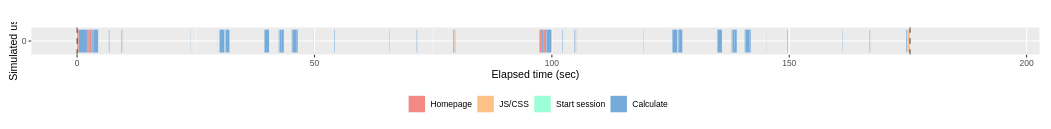
\includegraphics[scale=.4]{paperWSCAD2021/figures/user_x64_1_worker.png}
  \caption{Resultado da execução do simulador no \emph{server}, tempo demandado em cada evento com 1 \emph{woker}}
  \label{x64_1wroker}
\end{figure}

\begin{figure}[htbp]
  \centering 
  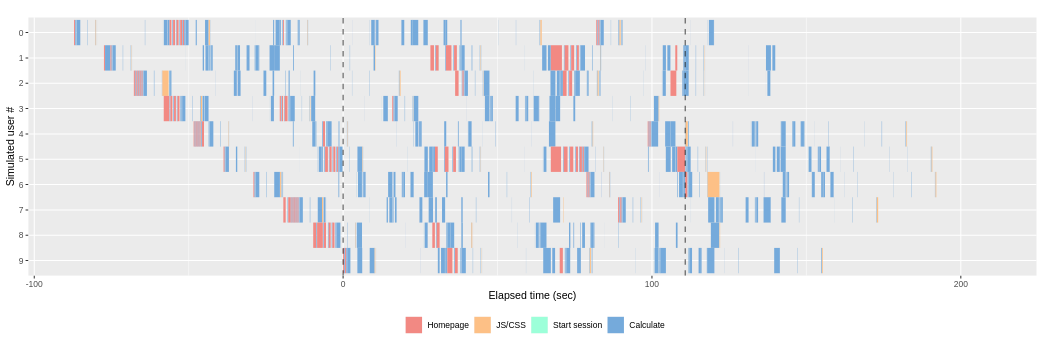
\includegraphics[scale=.4]{paperWSCAD2021/figures/user_x64_10_worker.png}
  \caption{Resultado da execução do simulador no \emph{server}, tempo demandado em cada evento com 10 \emph{woker}}
  \label{x64_10wroker}
\end{figure}

\begin{figure}[htbp]
  \centering 
  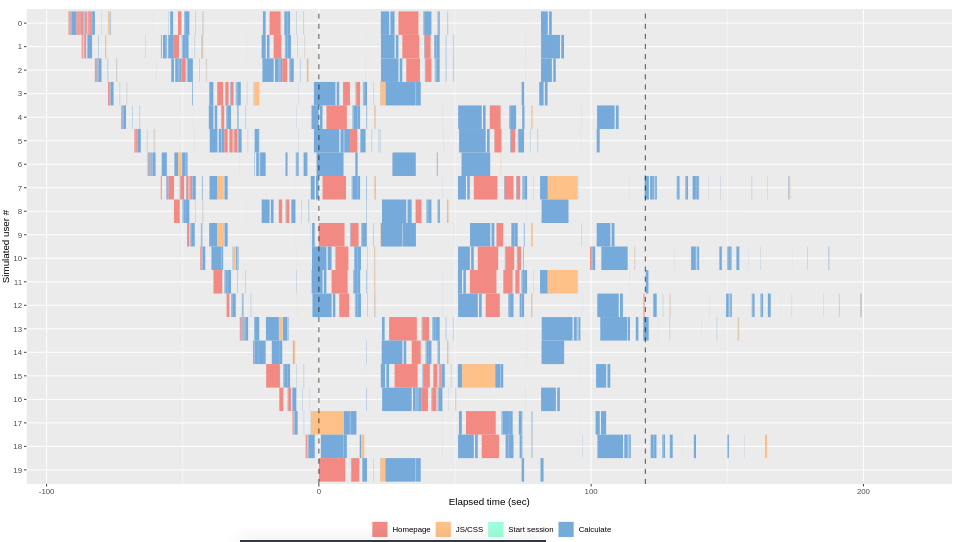
\includegraphics[scale=.4]{paperWSCAD2021/figures/user_x64_20_worker.png}
  \caption{Resultado da execução do simulador no \emph{server}, tempo demandado em cada evento com 20 \emph{woker}}
  \label{x64_20wroker}
\end{figure}

\begin{figure}[htbp]
  \centering 
  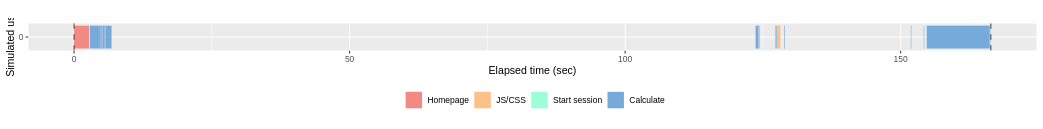
\includegraphics[scale=.4]{paperWSCAD2021/figures/user_PI3_1_worker.png}
  \caption{Resultado da execução do simulador na Raspberry PI3, tempo demandado em cada evento com um \emph{woker}}
  \label{PI3_1wroker}
\end{figure}

\begin{figure}[htbp]
  \centering 
  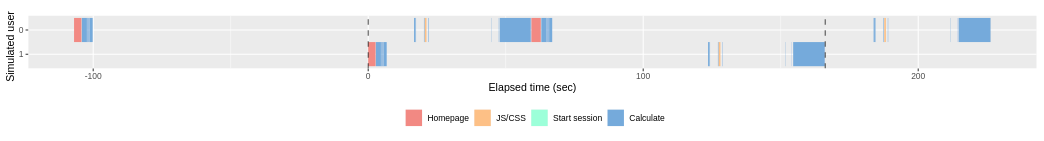
\includegraphics[scale=.4]{paperWSCAD2021/figures/user_PI3_2_worker.png}
  \caption{Resultado da execução do simulador na Raspberry PI3, tempo demandado em cada evento com um \emph{woker}}
  \label{PI3_2wroker}
\end{figure}

\begin{figure}[htbp]
  \centering 
  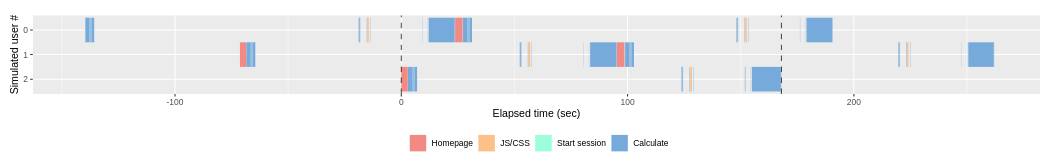
\includegraphics[scale=.4]{paperWSCAD2021/figures/user_PI3_3_worker.png}
  \caption{Resultado da execução do simulador na Raspberry PI3, tempo demandado em cada evento com três \emph{woker}}
  \label{PI3_3wroker}
\end{figure}

\begin{figure}[htbp]
  \centering 
  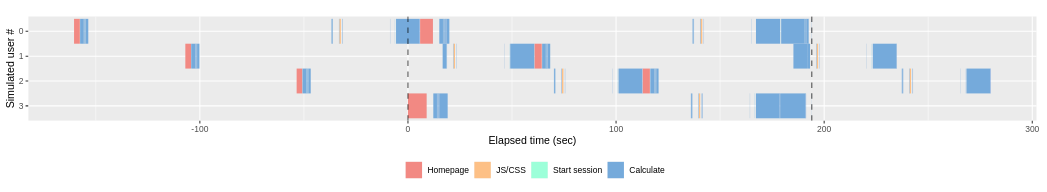
\includegraphics[scale=.4]{paperWSCAD2021/figures/user_PI3_4_worker.png}
  \caption{Resultado da execução do simulador na Raspberry PI3, tempo demandado em cada evento com quatro \emph{woker}}
  \label{PI3_4wroker}
\end{figure}

\section{Conclusão} \label{sec:conlusao}
De acordo a seção anterior, a Raspberry Pi 3 mostrou-se de certa forma eficiente para as execuções de um baixo número de usuários simultâneos, porém sendo pouco aproveitado do tempo de ociosidade do \emph{hardware}, o que permitiria assim, acrescentar mais usuários. 

Semelhantemente o \emph{server} apresentou um bom empenho como esperado para usuários simultâneos. Vale ressaltar que todos os testes aqui executados não contam com técnicas de \emph{tuning} para melhor escalonamento, utilizando assim toda configuração \emph{default} fornecida pela ferramenta, dessa forma, resultados diferentes podem ser obtidos quando melhores explorados.

Com tais dados, pudemos demonstrar a capacidade da Raspberry PI 3 em atender a aplicação de forma pessoal, ou seja, um atendimento interno a poucos usuários simultâneos. Demonstrando também a viabilidade de atendimento a um número maior de usuários, dado a ociosidade do \emph{hardware} quando já alcançado o limite indicado pelo simulador.

Com isso, como trabalhos futuros, pretende-se fazer uso de técnicas de \emph{tuning} para um novo teste de melhor aproveitamento da Raspberry PI3. Também pretende-se propor a recodificação da aplicação utilizando o modelo de arquitetura de micro serviços, dado sua orquestração permitida assim conseguindo escalonar de melhor forma, acredita se conseguir assim, extrair o máximo que o \emph{hardware} tem a oferecer sem a necessidade de reduzir a aplicação. 


\bibliographystyle{sbc}
\bibliography{sbc-template}

{\colo{red}\textbf{Retirado da Introdução:}
%Métricas de controle de qualidade e resultados ajudam a avaliar a confiança das previsões em estudos individuais.
R é uma ferramenta livre que oferece grande potencial para manipulação e visualização de massas de dados. Shiny é um pacote para R que permite que servidores disponibilizem recursos para visualizações R. 
%Existem outras, X e Y, que oferecem soluções semelhantes, porém, em um contexto proprietário.  
Com arquitetura igualmente livre, a placa Raspberry Pi - um minicomputador que tem todo o seu hardware integrado em uma placa única, inicialmente desenvolvida em 2006 por Eben Upton e equipe, %(Werner 2015) - 
possui um custo baixo de aquisição, tamanho pequeno e baixo consumo energético. Ela é versátil, podendo ser usado para os mais diferentes tipos de aplicações, inclusive provendo serviços nativos a servidores (dados, \emph{web}, serviços). 
%Um dado interessante é que o Raspberry Pi 3 foi selecionado como o SBC (single board computer) mais popular, entre 81 placas Linux / Android, numa pesquisa abrangente conduzida pela Linux Foundation em 2016 (Brown, 2016.
Equipamentos servidores, independentemente das tarefas a que são submetidos, demandam consumo energético constante e ininterrupto e, por óbvio, é interessante buscar soluções que reduzam o uso de energia, provendo assim economia ou ganho financeiro. }

\end{document}
